\vspace{-0.1cm}
\section{Experimental Results}
\vspace{-0.1cm}
\label{sec:results}


% \begin{figure}[t]
%     \centering
%     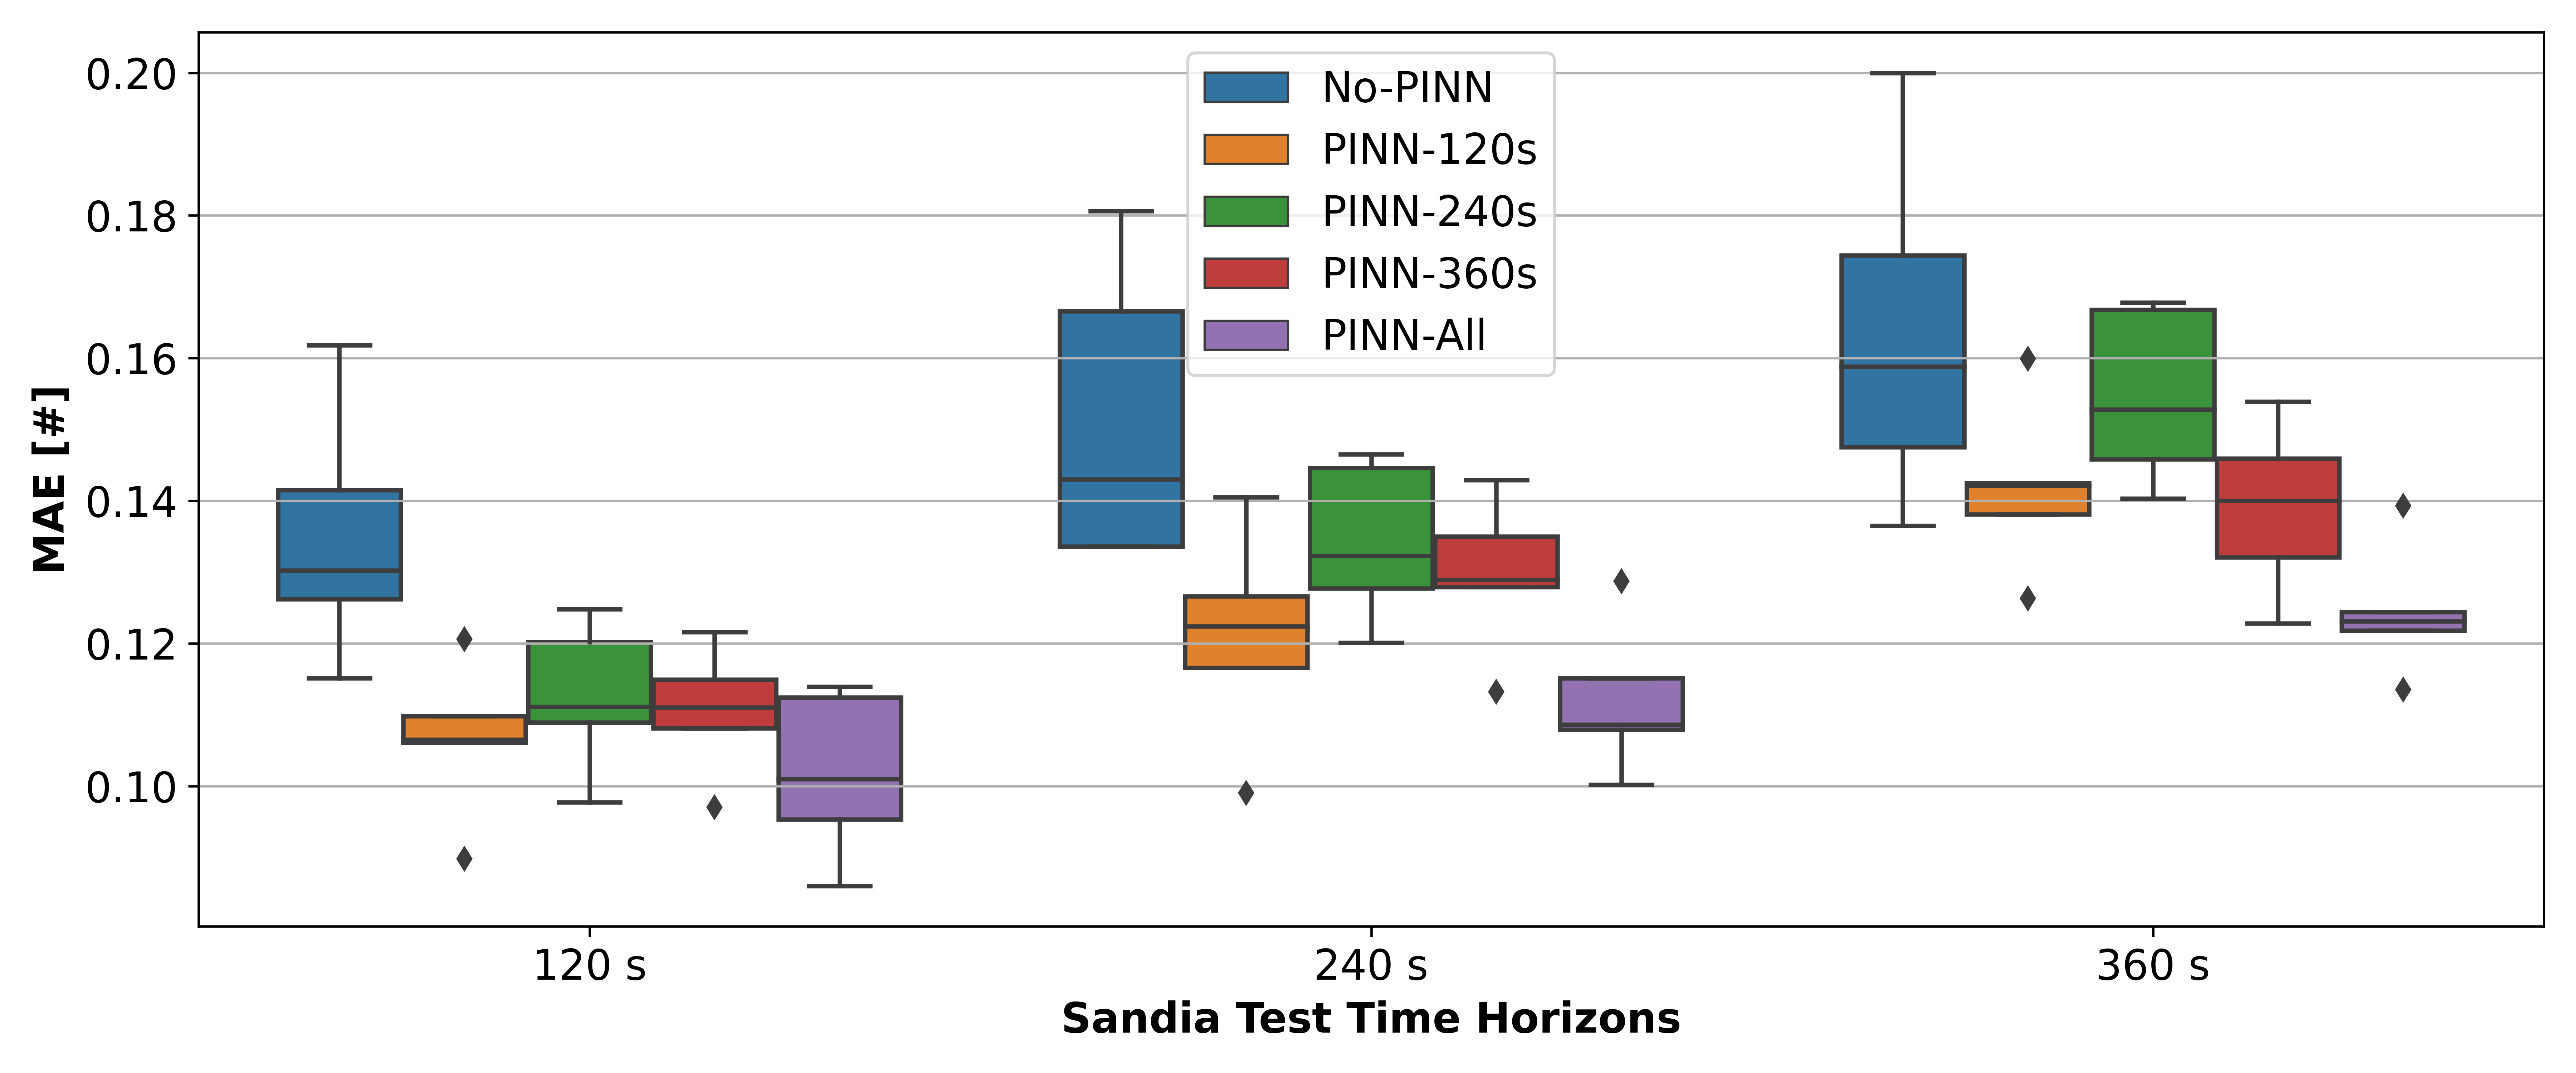
\includegraphics[width=.99\linewidth]{images/Sandia.png}
%     \caption{Results on Sandia dataset with different physic loss.}
%     \label{fig:sandia}
% \end{figure}

%\begin{figure}[t]
%    \centering
%    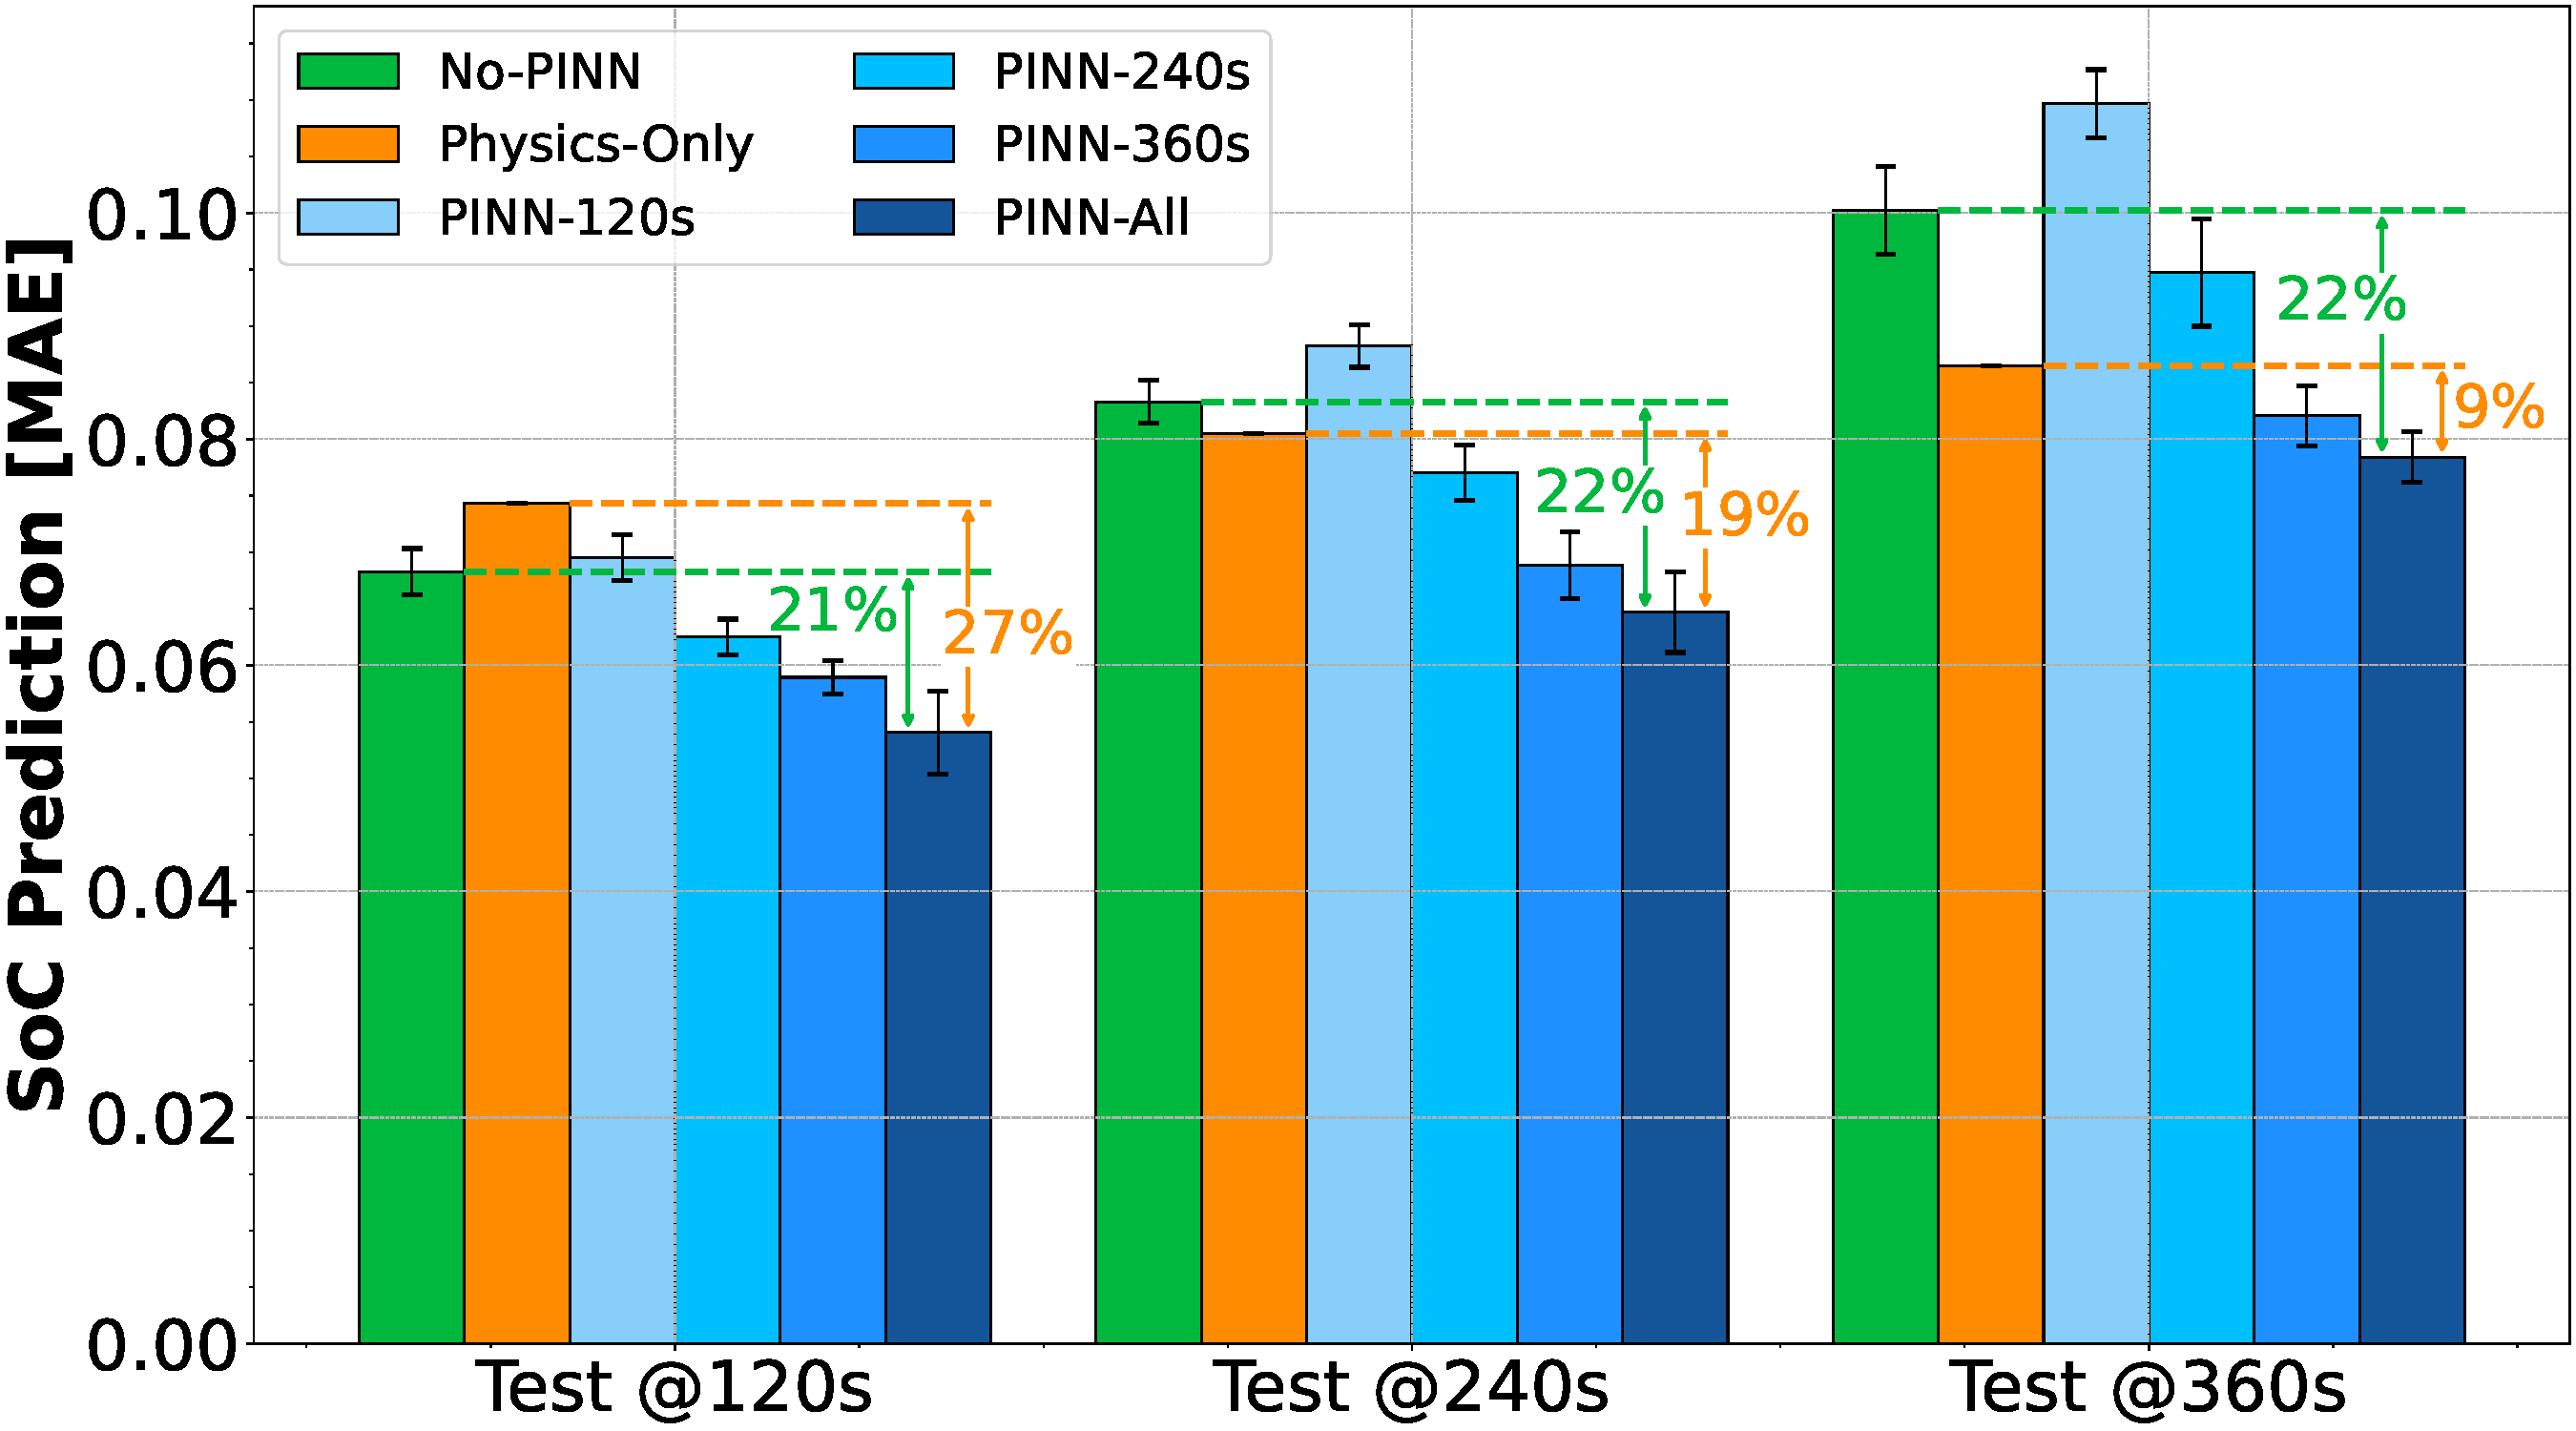
\includegraphics[width=0.99\linewidth]{images/sandia-new.pdf}
%    \vspace{-0.5cm}
%    \caption{Results on Sandia dataset with different physic loss}
%    \vspace{-0.5cm}
%    \label{fig:sandia}
%\end{figure}
%This section presents the results. 
\subsection{Results on the Sandia Dataset}
\vspace{-0.1cm}
We first benchmark our proposed network on the Sandia Dataset, showing the network performance on the three test conditions described in the previous section.
Figure \ref{fig:sandia} shows the overall results in terms of SoC prediction MAE. 
% \st{Each group of results on the x-axis corresponds to a test dataset with a different time horizon (120s, 240s and 360s, respectively). The five box plots in each group correspond to the different No-PINN/PINN configurations.}
The x-axis groups the results by test dataset, each corresponding to a different time horizon (120s, 240s, and 360s, respectively). Within each group, each of the 6 bars represents a specific configuration of the physics loss. Physics-Only is a model whose second branch predicts the SoC \textit{exclusively} employing Eq.~\ref{eq:cc} (without using training data at all). The individual bars within each subgroup average the results over 5 runs with different random seeds.

The first thing to notice is that the No-PINN solution (trained only on 120s-spaced data points) is outperformed in  every test condition.  This demonstrates the regularizing effect of the physics loss component, which improves the generalization of the model even under the same time horizon used for the training data.
%
The No-PINN baseline obtains a MAE of 0.068, 0.083, and 0.1 for the three different time horizons, 
% \st{being outperformed by 1.33x, 1.35x, and 1.31x respectively by the best PINN solution.} 
being outperformed by 21\%, 22\%, and 22\% respectively by the best PINN.
Interestingly, we find that the PINN trained using all time horizons simultaneously in the physics loss (PINN-All) achieves the best performance for all test conditions, even outperforming the ones whose physics loss includes solely examples with $N_p$ equal to the tested horizon. This result suggests that giving multiple $N_p$ values to the physics equations let the network learn better the underlying relation between SoC, time, current and temperature.
%
In contrast, training Branch 2 using the physics loss coupled with \textit{single values} of $N_p >$ 120s does not always lead to an advantage.
%
Moreover, comparing the performance of PINN-All to Physics-Only reveals a consistent improvement across all scenarios. This underscores how the NN, even more when augmented with the physics component, excels at extracting valuable features from raw data, thereby significantly enhancing the model's accuracy.
%
% \revtwo{This phenomenon is probably due to the fact that, for the Sandia dataset, the current is approximately constant and the network learns only to associate the SoC estimation to the time elapsed. Therefore, the non-linear behavior of charge/discharge cycle which should be extrapolated from the training dataset is not learned by the network and the overall MAE increases. \textbf{DP: non mi convince questa giustificazione}}

%\begin{figure}[t]
%    \centering
%    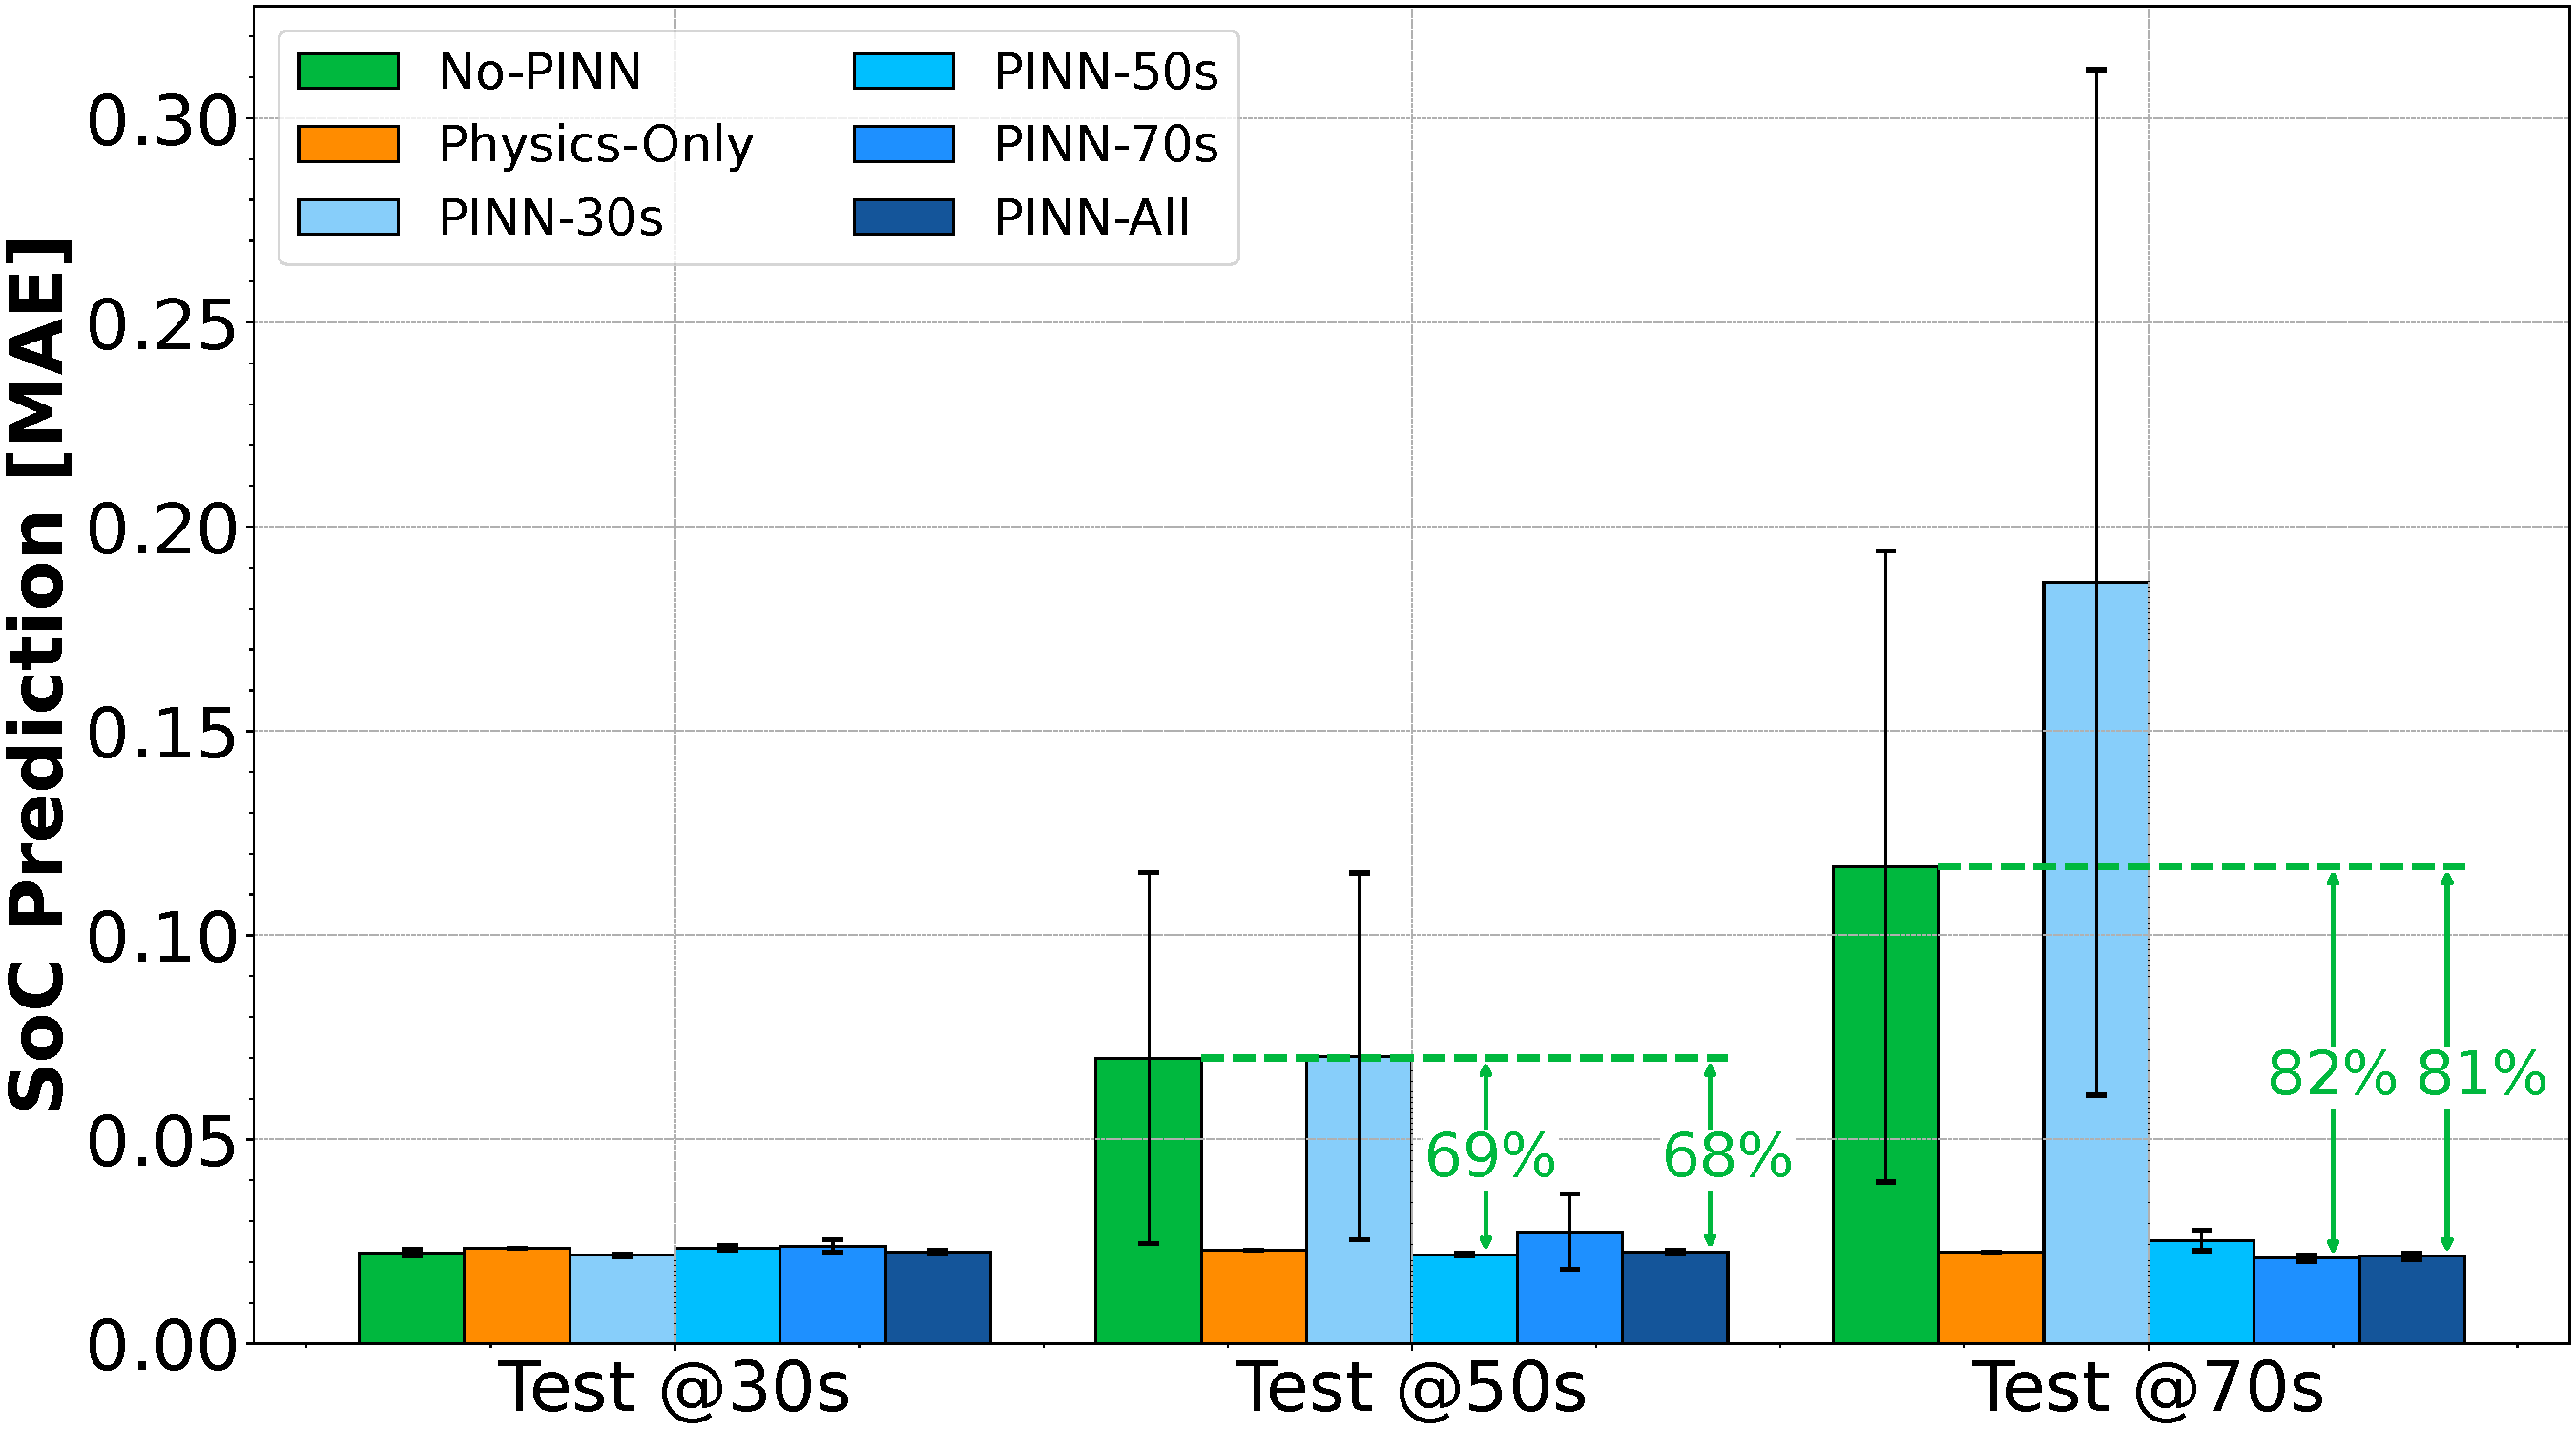
\includegraphics[width=.99\linewidth]{images/lg-new.pdf}
%    \vspace{-0.5cm}
%    \caption{Results on LG dataset with different physic loss}
%    \vspace{-0.6cm}
%    \label{fig:LG}
%\end{figure}
\subsection{Results on the LG Dataset}
\label{sec:lg-results}
Given the limited charge/discharge conditions (i.e., constant current) of the Sandia dataset, we also benchmark our approach on the LG dataset, which contains more complex charge and discharge patterns with varying currents.
Figure \ref{fig:LG} illustrates the result for this dataset with a visualization analogous to the previous section, but using 30, 50, and 70 seconds as prediction horizons.
It is worth observing that for this dataset, contrary to the previous one, the PINN trained with $N_p$ equal to the time horizon used for testing always achieves the best result on the corresponding test condition. 
%
Namely, they achieve 0.0217, 0.0218, and 0.0210 MAE on the predicted SoC, outperforming the No-PINN result by 3\%, 69\%, and 82\%, respectively.
%
However, similarly to the Sandia experiments, using the physics equation with multiple time horizons simultaneously (PINN-All), allows the network to closely approach the best performance in all test conditions. 
%
In particular, PINN-All achieves the second lowest MAE overall of 0.0214, being just 1.8\% less accurate than the best model (PINN-70s).
%
This shows that the physics loss allows the network to better generalize even when charge and discharge currents change over time.
% \st{The best PINNs for each test condition achieve 0.0128, 0.0129, and 0.0133 MAE on the predicted SoC, outperforming the network trained without the physics data by 1.13x, 2.97x, and 4.36x respectively.}
% Also note that the more the time horizon increases, the larger the error of the No-PINN architecture, suggesting that the inclusion of the physics equation becomes more important.

% \st{It is also interesting to notice that the larger is the $N_p$ value, the lower becomes the overall MAE, in all three test conditions, confirming an improved generalization of the network when the physics equation is used to generate data farther from the dataset ones.}
%%%%%%%%%%%%%%%%%
%%% OLD TABLE %%%
%%%%%%%%%%%%%%%%%

% \begin{table}[]
% \caption{Comparison with SoA on the LG dataset.}
% \label{tab:soa}
% \begin{tabular}{l|lll}
% \hline
%                                  & T {[}°C{]} & SoC Estimation & SoC Pred. \\ \hline
% Our Work (No PINN)               & 25         & 0.013         & 0.038           \\
% Our Work (PINN-All)              & 25         & 0.013         & 0.013           \\ \hline
% LSTM~\cite{wong-2021}    & 25         & 0.012          & n.a.            \\
% LSTM~\cite{wong-2021}    & 0          & 0.017          & n.a.            \\
% DE-LSTM~\cite{Dang23} & 0          & 0.129          & n.a.            \\
% DE-MLP~\cite{Dang23} & 0          & 0.177          & n.a.            \\ \hline
% \end{tabular}
% \end{table}

%%%%%%%%%%%%%%%%%
%%% NEW TABLE %%%
%%%%%%%%%%%%%%%%%
%\begin{table}[]
%\footnotesize
%\vspace{-0.2cm}
%\caption{Comparison with SoA on the LG dataset for the prediction of SoC(t) and SoC(t+N)}
%\label{tab:soa}
%\begin{tabular}{l|lllll}
%\hline
%                                 & T {[}°C{]} & SoC(t) & SoC(t+N) & Mem & %Ops\\ \hline
%No-PINN               & 0         & 0.031         & 0.036 & $\simeq$ 9kb %&     $\simeq$ 1150    \\
%No-PINN               & 25         & 0.014         & 0.016 & $\simeq$ 9kb %&     $\simeq$ 1150    \\
%PINN-All              & 0         & 0.031         & 0.032 & $\simeq$ 9kb  %& $\simeq$ 1150       \\
%PINN-All              & 25         & 0.014         & 0.014 & $\simeq$ 9kb % & $\simeq$ 1150       \\ \hline
%LSTM~\cite{wong-2021}    & 25         & 0.012          & n.a.         & $\simeq$ 4Mb& $\simeq$300M  \\
%LSTM~\cite{wong-2021}    & 0          & 0.017          & n.a.           & $\simeq$4Mb & $\simeq$300M\\
%DE-LSTM~\cite{Dang23} & 0          & 0.129          & n.a.            & n.a. & n.a.\\
%DE-MLP~\cite{Dang23} & 0          & 0.177          & n.a.            & n.a. & n.a.\\ \hline
%\end{tabular}
%\vspace{-0.4cm}
%\end{table}
It is also noteworthy that as the value of $N_p$ increases, the error of the No-PINN architecture grows, and the overall improvement in MAE due to physics becomes more pronounced. This confirms the importance of the physics loss in regularization, especially when dealing with data farther from the training dataset.
\vspace{-0.25cm}
\subsection{State-of-the-art Comparison}
\vspace{-0.1cm}
In this section, we focus on the LG dataset to compare our proposed approach with the best SoA algorithm for SoC estimation \cite{wong-2021} and with \cite{Dang23}, that is the most similar work to ours (as presented in Sec. \ref{sec:background}, as it also exploits physics equations during training).%, on the LG dataset.

Table \ref{tab:soa} reports the results obtained on SoC estimation, i.e., the error on SoC(t), computed with data measured from the battery, and on SoC prediction, i.e., the error on SoC(t+N). 
%
%computed using the estimated battery usage in the time period t to t+N.
%
For our method, we report the output of Branch 1 for the former, and of the full network for the latter,
%
% \st{The latter result is reported as the average of the performance achieved with the 30s, 50s, and 70s time horizons (see previous section).}
using a 30s time horizon.
%
% \revtwo{Note that, to the best of our knowledge, our work is the first to explore the task of predicting the future SoC given a target workload, showing an impressive SoC prediction MAE of 0.013 when exploiting physics equations to train the network.}
Note that none of the previous works tested on this dataset have considered the prediction of future SoC values. Our work addresses this more complex task, achieving an impressive SoC prediction MAE of 0.014 when exploiting physics equations to train our networks.
Moreover, we also demonstrate comparable performance on the same task of the SoA, i.e., the instantaneous SoC estimation.
When compared to \cite{wong-2021}, our approach reaches almost the same MAE (0.014 vs. 0.012) on the same test dataset, with a model that requires an impressive 260k$\times$ fewer operations and 400$\times$ less memory.
Compared to \cite{Dang23}, we obtain 4.2$\times$ lower MAE than their best solution, an LSTM with comparable dimensions of the one of~\cite{wong-2021}, and up to $\simeq$6$\times$ lower MAE when compared to their proposed MLP architecture.
We argue that we achieve better performance thanks to the introduced moving average on input windows, used as pre-processing before feeding the data to Branch 1. This allows the network to account for I, V, and T information of the last 30 seconds instead of their noisy instantaneous values.
% \vspace{-0.1cm}
\subsection{Full discharge analysis}
%\begin{figure*}[ht]
%    \centering
%    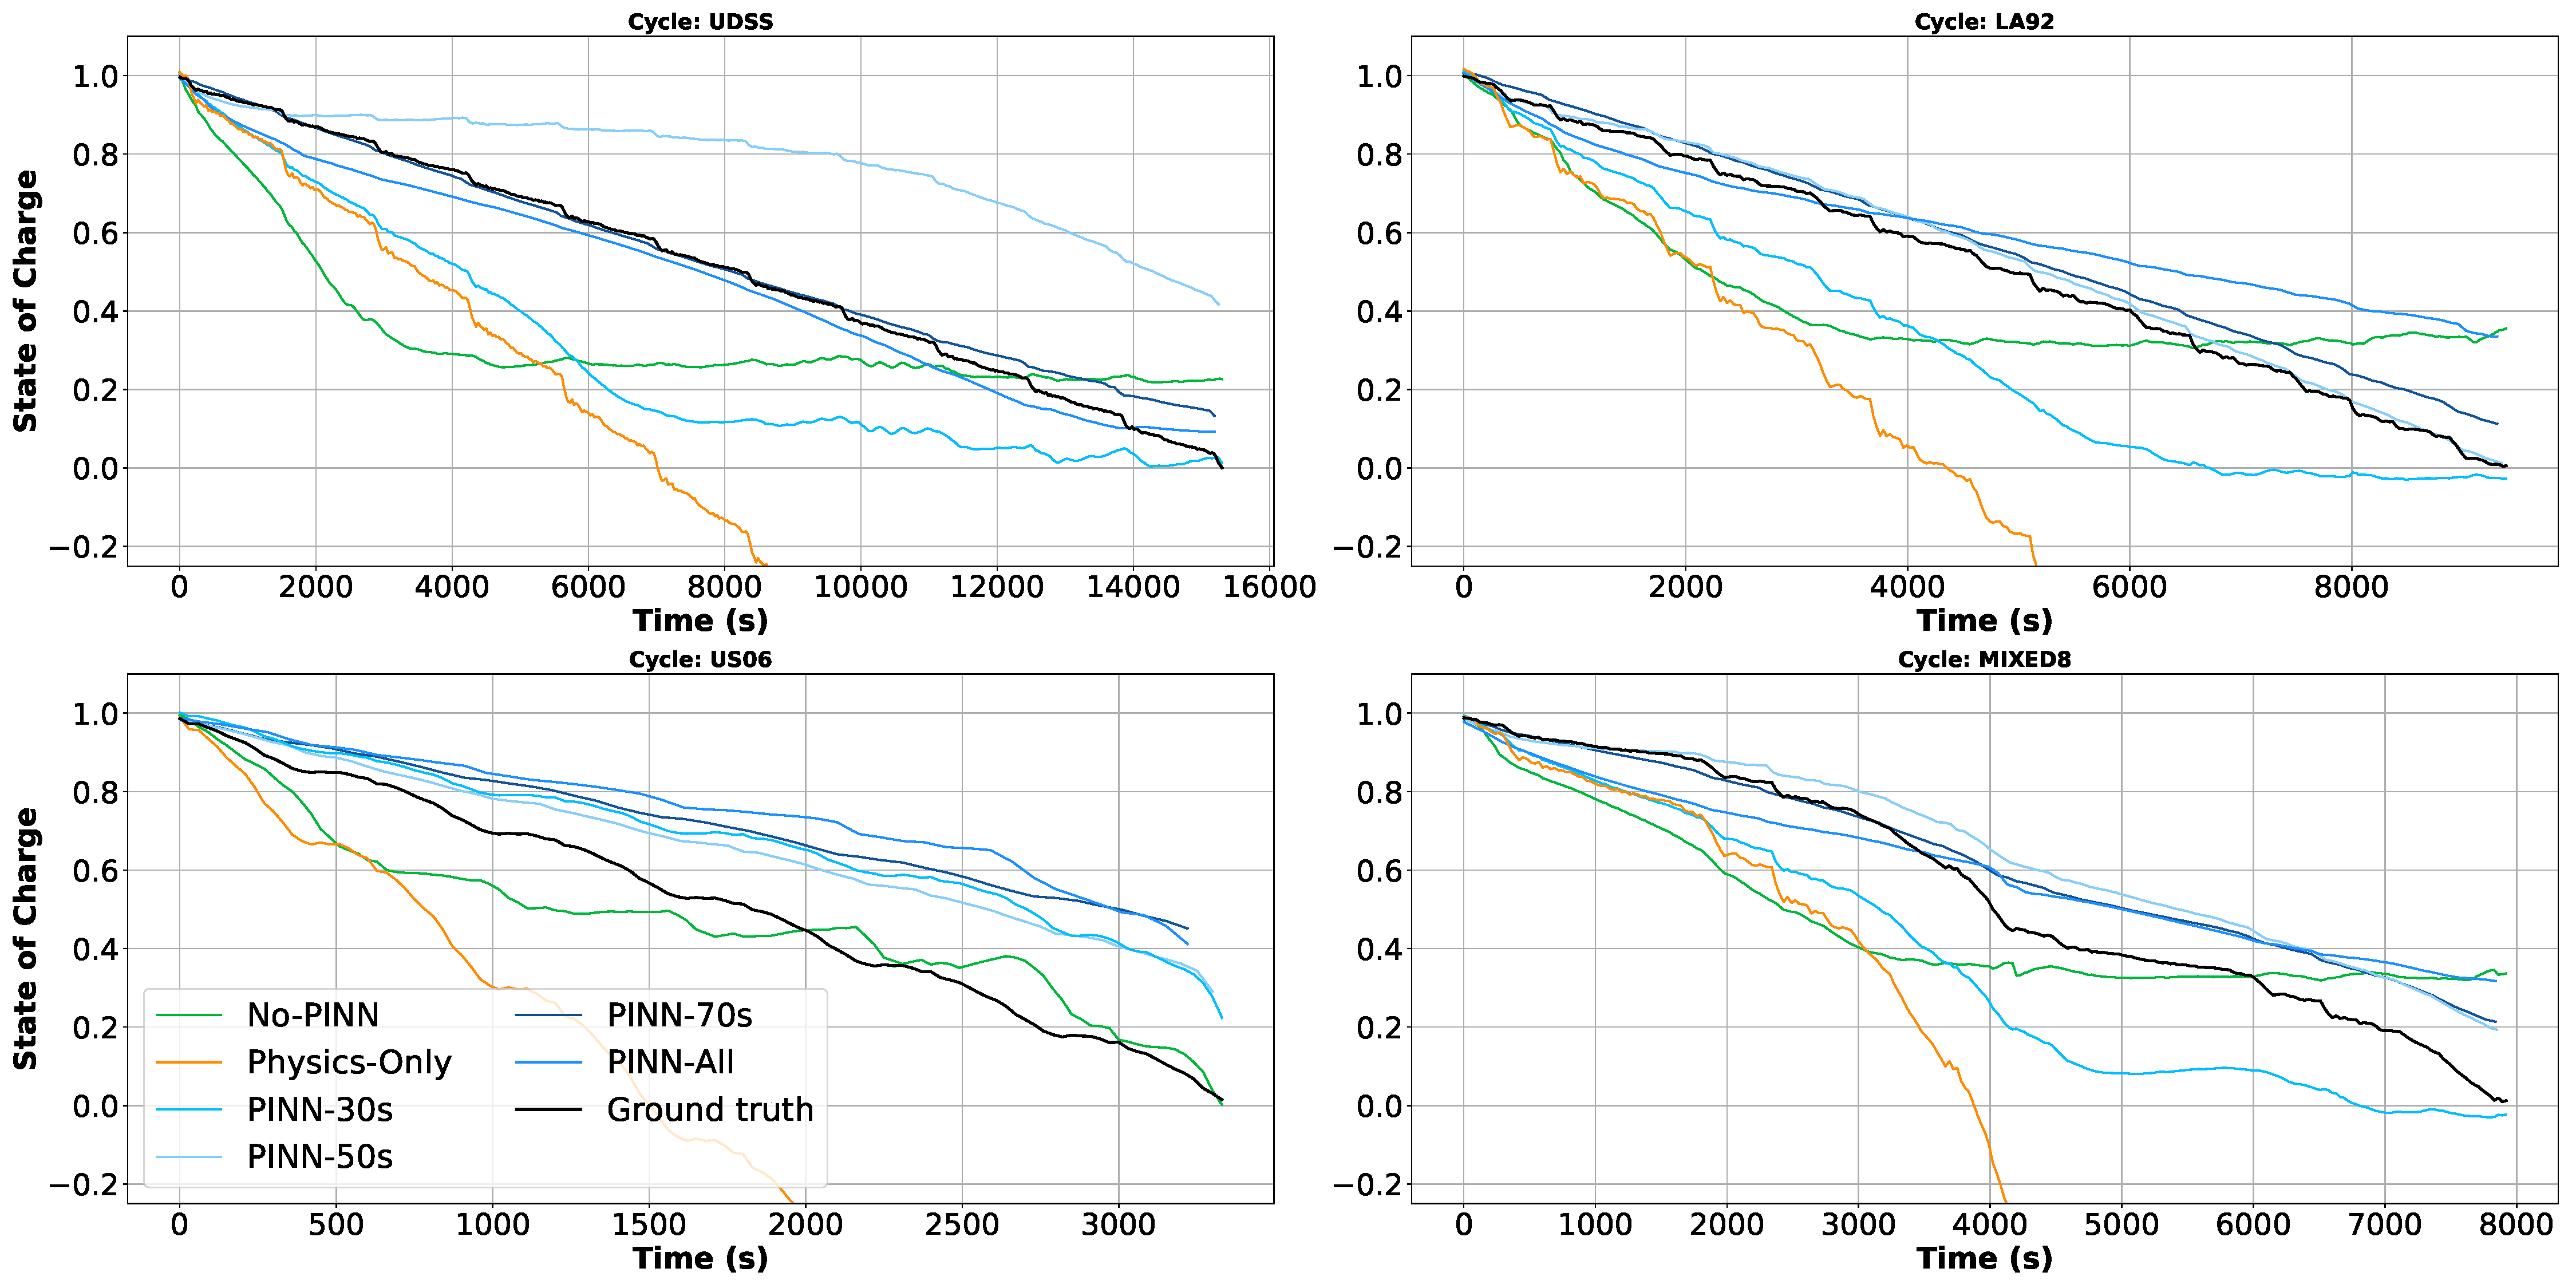
\includegraphics[width=\linewidth]{images/Battery_Cycles_Subplots_with_Output.pdf}
%    % \vspace{-0.4cm}
%    \caption{Auto-regressive inference with our networks, on the four driving cycles of the LG dataset, at 25°C.}
%    \vspace{-0.2cm}
%    \label{fig:full-discharge}
%\end{figure*}
In this final section, we illustrate the estimation of a complete discharge cycle, leveraging the autoregressive application of our model, depicted in Fig.~\ref{fig:nn-autoregressive}. We target the entire four ``driving'' cycles of the LG test dataset. 
We highlight that this is a critical task, i.e., predicting the battery lifetime given a target workload, that can not be solved by SoA methods, given that they require instantaneous voltage information, whereas we use voltage as input \textit{only at the first timestamp}.
% On the other hand, solving this task allows for the prediction of the battery lifetime given a target workload and, therefore, its optimization.
In Fig. \ref{fig:full-discharge}, each line represents a different network configuration. For all models, the single-step time horizon for SoC prediction is set as the one that resulted in the lowest MAE in the previous experiments. Then, multiple autoregressive predictions are performed. For instance, for the PINN-50s, we use 50 seconds as the time horizon: we first predict SoC(0) with Branch 1, and then recursively use Branch 2 to predict SoC(50), SoC(100), etc.
The black line represents the golden SoC of the battery. 
% \st{The No-PINN configuration uses predictions with a time horizon of 30s, corresponding to the same value of $N$ seen during training, and to its best testing condition (see Fig.5).}
The No-PINN and the Physics-Only configurations use a time horizon of 30s, corresponding to the same value of $N$ present in the dataset, and to their best testing condition (see Fig. \ref{fig:LG}).
The first thing that we notice is that the No-PINN architecture achieves poor performance on SoC prediction for 3 out of 4 cycles. 
Similarly, the Physics-Only approach consistently performs the worst among all cycles. This is primarily because errors accumulate with each iteration, and without accounting for voltage in the equation, the predictions tend to diverge rapidly. Interestingly, while values are overestimated, the \textit{shape} of the discharge patterns predicted by Physics-Only closely align with the ground truth, hinting at why incorporating the physics equation during training can enhance performance.
Indeed, combining physics and data-driven training strongly improves the results, stepping from an average final SoC prediction of 0.234 (ground truth is SoC=0.0) for the No-PINN case to 0.089 for the best PINN setup, i.e., PINN-30s. 
The only cycle where the PINNs marginally underperform is the US06.
Importantly, the higher errors shown in this experiments are due to accumulation caused by the autoregressive inference,
demonstrating that this task is much more challenging compared to the estimation of the instantaneous SoC, or to the prediction of the SoC at a single future time instant.
%
However, we note that running an autoregressive prediction that lasts for a full discharge cycle is an extreme case, that would probably not occur in practice. A more realistic usage of our model would run a limited number of autoregressive steps, depending on the length of the workload whose effect on the SoC shall be predicted, thus, limiting the error accumulation.

